\documentclass[a4paper]{article}

\usepackage[english]{babel}
\usepackage[utf8x]{inputenc}
\usepackage{amsmath}
\usepackage{graphicx}
\usepackage{algorithm}
\usepackage{algorithmicx}
\usepackage{algpseudocode}
\usepackage{url}
\renewcommand{\algorithmicforall}{\textbf{for each}}
\let\ForEach\ForAll

\title{ParMA Partition Improvement with Ghosting}

\author{Cameron W. Smith, Gerrett Diamond, Dan Ibanez}

\date{\today}

\begin{document}
\maketitle

\section{Problem Description}

A climate application's pre-processor has a runtime proportional to the number of owned elements plus the number of ghost elements in three ghosting layers; the ghost bridge entity is an edge.  2D meshes of the ocean surface are created using Spherical Centroidal Voronoi Tesselations ~\cite{JuRingler2011,ringler2008}.  The goal is to partition this mesh such that Equation~\ref{eqn:costFn} is minimized while maintaining a low edge cut.  Here the notation $M^d$ is a mesh element and $gM^d$ is a ghost mesh element.
\begin{equation}
\label{eqn:weightVoroni}
w(p_i) = \sum_{M^d \in p_i}w(M^d) + \sum_{gM^d \in p_i}w(gM^d)
\end{equation}
\begin{equation}
\label{eqn:costFn}
I = \frac{max(w(p))}{avg(w(p))}
\end{equation}
Most partitioners cannot account for the ghosted elements as the affect of the ghosts on $w(p_i)$ changes with the partitioning of the owned elements.  

Figure~\ref{fig:ghostEx} depicts an example of three layer ghosting in the polyhedral mesh.

\begin{figure} 
\centering
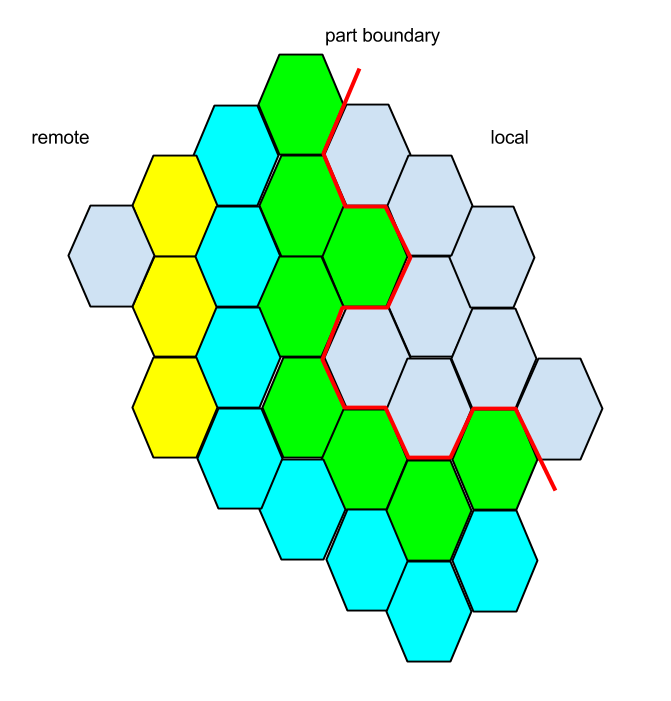
\includegraphics[width=0.4\textwidth]{ghostingExample.png}
\caption{\label{fig:ghostEx} Three layers of elements ghosted from the remote part to the local part.  The first layer is colored green, the second blue, and the third yellow.}
\end{figure}

\section{Approach}

ParMA diffusive partition improvement procedures can account for the ghosted layers using a combination of existing element selection criteria and an extended 'weight' tracking mechanism.  The weight tracking extension relies on the exact knowledge of the change to the ghosted elements as elements on a heavy part are selected for migration to a light part.

ParMA will be ran on the delaunay trianularization of the Voronoi mesh (Figure~\ref{fig:delaunay}), as depicted in Figures~\ref{fig:NA240}, \ref{fig:east60}, and \ref{fig:NA60}, and will accordingly target vertex balance.  The vertex part assignments, along with identifier information, will be output for partitioning the Voronoi mesh. Vertices in the initial partition are identified by their part number and local vtx number.  Details on the meshes of interest are available online ~\cite{climateMesh}. 

\begin{figure} 
\centering
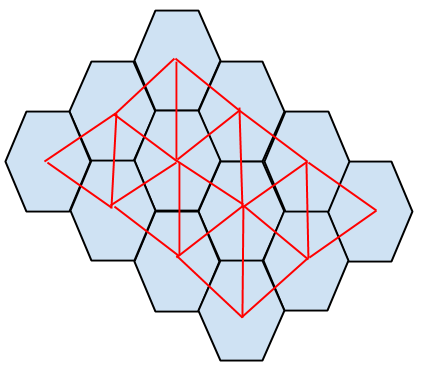
\includegraphics[width=0.4\textwidth]{ghostingOwnershipFig1.png}
\caption{\label{fig:delaunay} A Voronoi diagram and its Delaunay triangularization (in red).}
\end{figure}

\begin{figure}
\centering
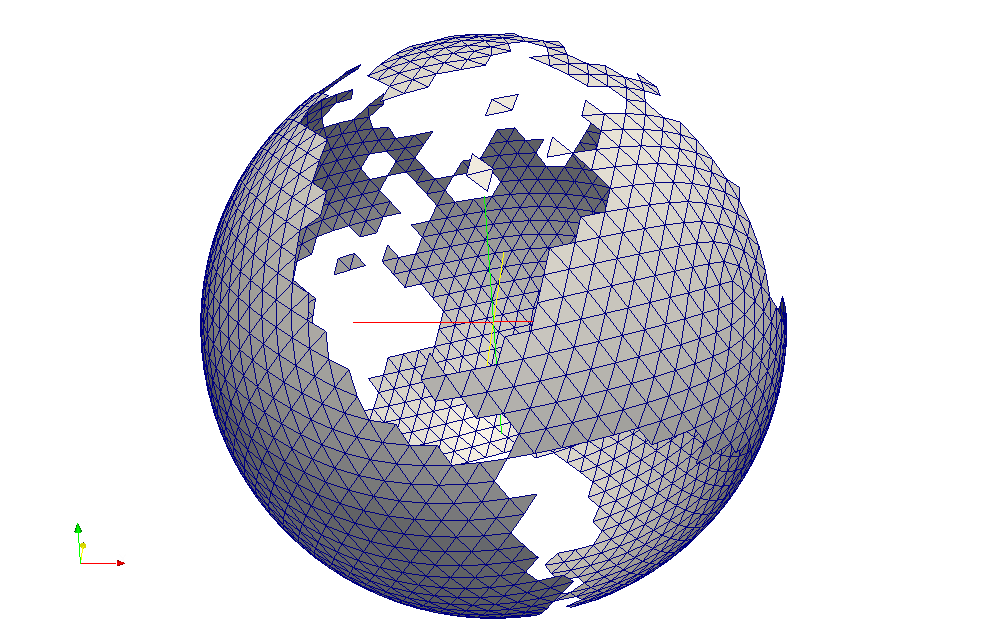
\includegraphics[width=0.75\textwidth]{ocean_QU_240kmNA.png}
\caption{\label{fig:NA240} 240km resolution dual mesh.}
\end{figure}

\begin{figure}
\centering
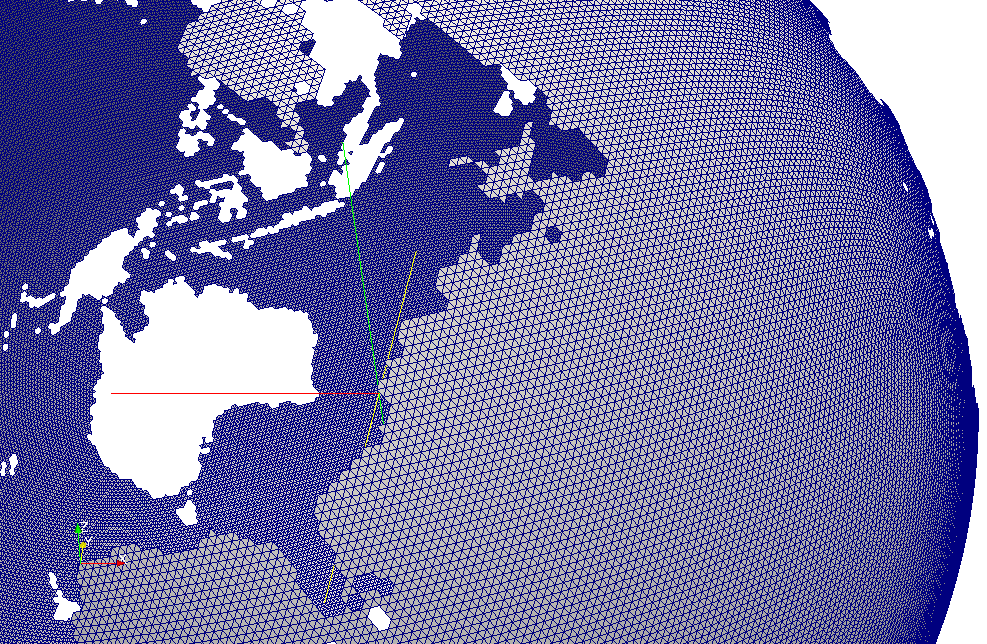
\includegraphics[width=0.75\textwidth]{ocean_QU_60kmNA_eastCoastZoom.png}
\caption{\label{fig:east60} 60km resolution dual mesh of North American east coast.}
\end{figure}

\begin{figure}
\centering
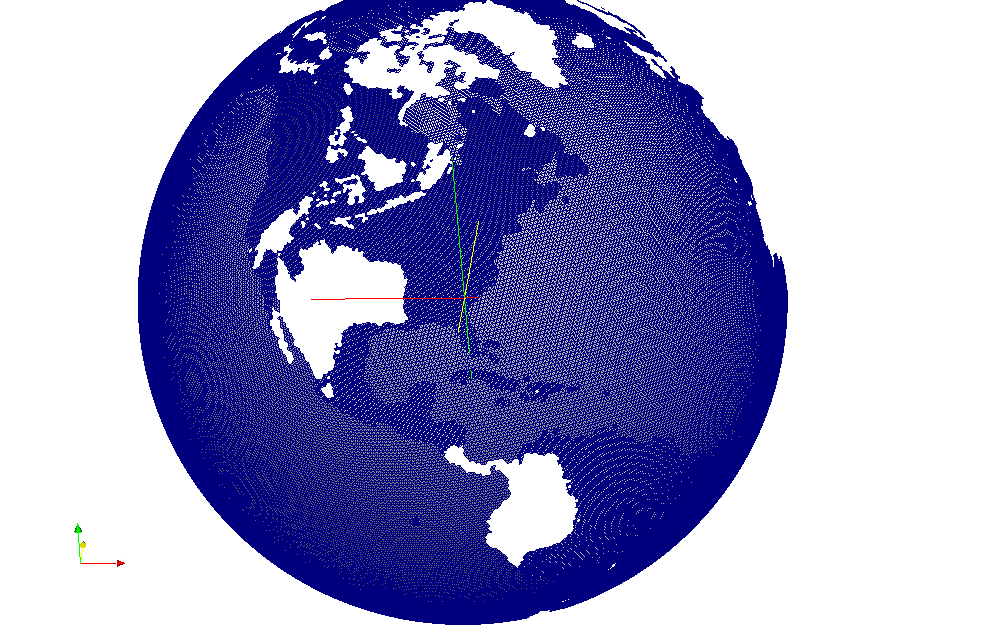
\includegraphics[width=0.75\textwidth]{ocean_QU_60kmNA_far.png}
\caption{\label{fig:NA60}60km resolution dual mesh.}
\end{figure}

A Delaunay mesh vertex based partitioning, as depicted in Figure~\ref{fig:ownership2}, is not a valid partition of the Delaunay mesh as each element needs to be assigned to exactly one part.  To obtain unique element assignment an element based partitioning of the Delaunay mesh is performed.  Duplicate Delaunay vertices created on the part boundary as a result of the element partitioning are depicted in Figure~\ref{fig:ownership3} by dotted lines.  These vertex copies in the Voroni mesh this correspond to an element assigned to multiple parts.  Unique part assignment of the Voroni mesh elements is through the ownership associated with the Delaunay mesh vertices.  In Figure~\ref{fig:ownership3} ownership of a mesh vertex is depicted through a colored Voroni element.  Using vertex ownership the weight of each part is defined in Equation~\ref{eqn:weightDelaunay}; the notation $M^0$ is a mesh vertex, $gM^d$ is a ghost mesh vertex, and $\hat{M^0}$ denotes the owned copy of the vertex.
\begin{equation}
\label{eqn:weightDelaunay}
w(p_i) = \sum_{\hat{M^0} \in p_i}w(\hat{M^0}) + \sum_{gM^0 \in p_i}w(gM^0)
\end{equation}

In the Voroni mesh the bridge entity is an edge and three layers of ghosts are needed.  For each shared Voroni mesh edge there is a Delaunay mesh edge connecting Delaunay mesh vertices.  Ghost Delaunay mesh vertices are located using a edge-depth three BFS with root nodes defined as owned Delaunay mesh vertices classified on the partition model boundary.  As with non-ghost Delaunay mesh vertices, each Delaunay mesh ghost vertex corresponds to a Voroni mesh element.  In Figure~\ref{fig:ownership4} the ghost depth is one and green elements are ghosted to the bottom part and yellow elements ghosted to the top part.  The first layer of vertices to be ghosted is formed by (1) the owned vertices classified on the part boundary and (2) vertices edge-adjacent to un-owned vertices classified on the part boundary.

Algorithm~\ref{alg:parma} outlines the top-level procedure for iterative diffusion that seeks to reduce $I$.  While the mesh peak imbalance $I$ is greater than the specified target imbalance a diffusive iteration is executed.  Each iteration first requires finding neighboring parts, computing part weights and exchanging those weights with neighboring parts, finding the elements ghosted on the part boundaries and exchanging the weight of those ghosts with neighboring parts, and lastly computing the amount of weight to migrate to each neighbor.  

\begin{figure} 
\centering
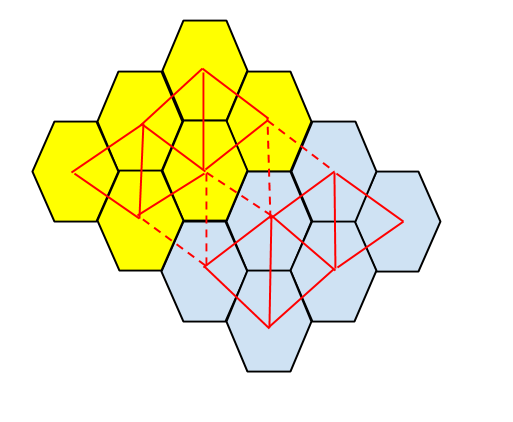
\includegraphics[width=0.4\textwidth]{ghostingOwnershipFig2.png}
\caption{\label{fig:ownership2} A Delaunay mesh vertex based partitioning is not a valid partition of the Delaunay mesh as elements, denoted with dashed edges, span the part boundary.  In the scorec unstructured mesh tools an element cannot be divided between multiple parts.}
\end{figure}

\begin{figure} 
\centering
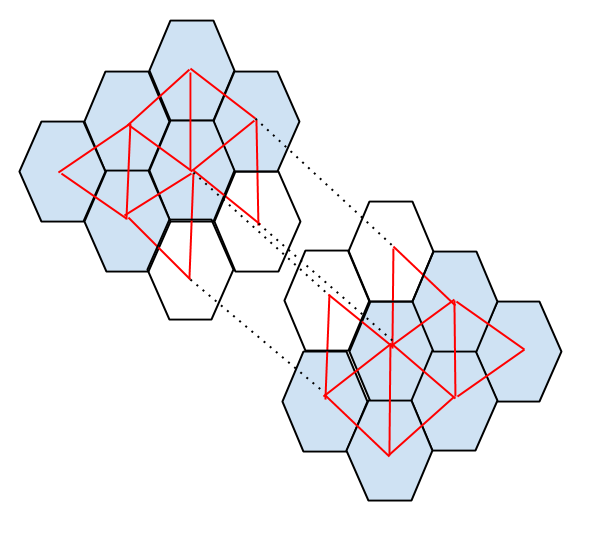
\includegraphics[width=0.4\textwidth]{ghostingOwnershipFig3.png}
\caption{\label{fig:ownership3} An element based partitioning of the Delaunay mesh with duplicate Delaunay vertices on the part boundary.  Owned Delaunay mesh vertices are marked with colored Voroni elements.}
\end{figure}

\begin{figure} 
\centering
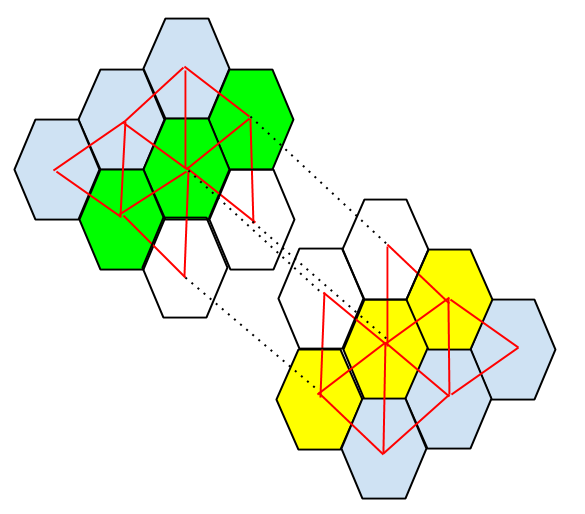
\includegraphics[width=0.4\textwidth]{ghostingOwnershipFig4.png}
\caption{\label{fig:ownership4} One layer edge-based ghosting of a Delaunay mesh element partition.  Green elements are ghosted to the bottom part and yellow elements ghosted to the top part.}
\end{figure}


\section{Results}

\begin{figure} 
\centering
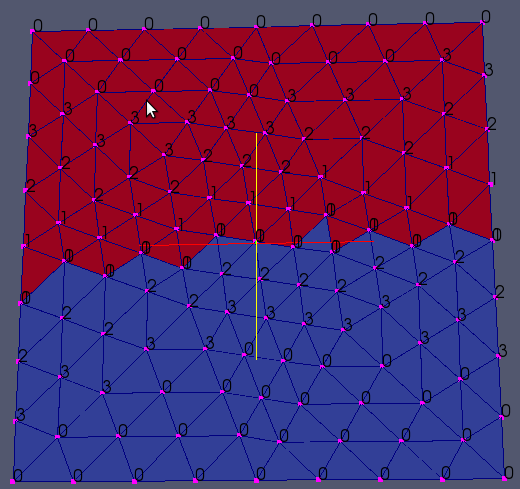
\includegraphics[width=0.8\textwidth]{plateghosts.png}
\caption{\label{fig:ownership4} Three layers of ghosting between two parts of a test mesh.  The boundary is only ghosted from the part that owns the vertices to the not owned part.}
\end{figure}

\begin{center}
\begin{tabular}{c | c | c | c}
  \hline
  parts & initial imbalance & final imbalance & parma-ghost runtime \\
  64 & 1.135 & 1.046 & 2.0222 \\
  128 & 1.158 & 1.040 & 1.2728 \\
  256 & 1.194 & 1.048 & 1.8081 \\
  512 & 1.348 & 1.058 & 1.7639 \\
  \hline 
\end{tabular}
\end{center}

Testing was done on AMOS with a 60km mesh of the ocean using 64 nodes with varying part numbers ranging from 64 to 512 parts. The method was repeated until imblance reached 1.05 or better.

\begin{figure} 
\centering
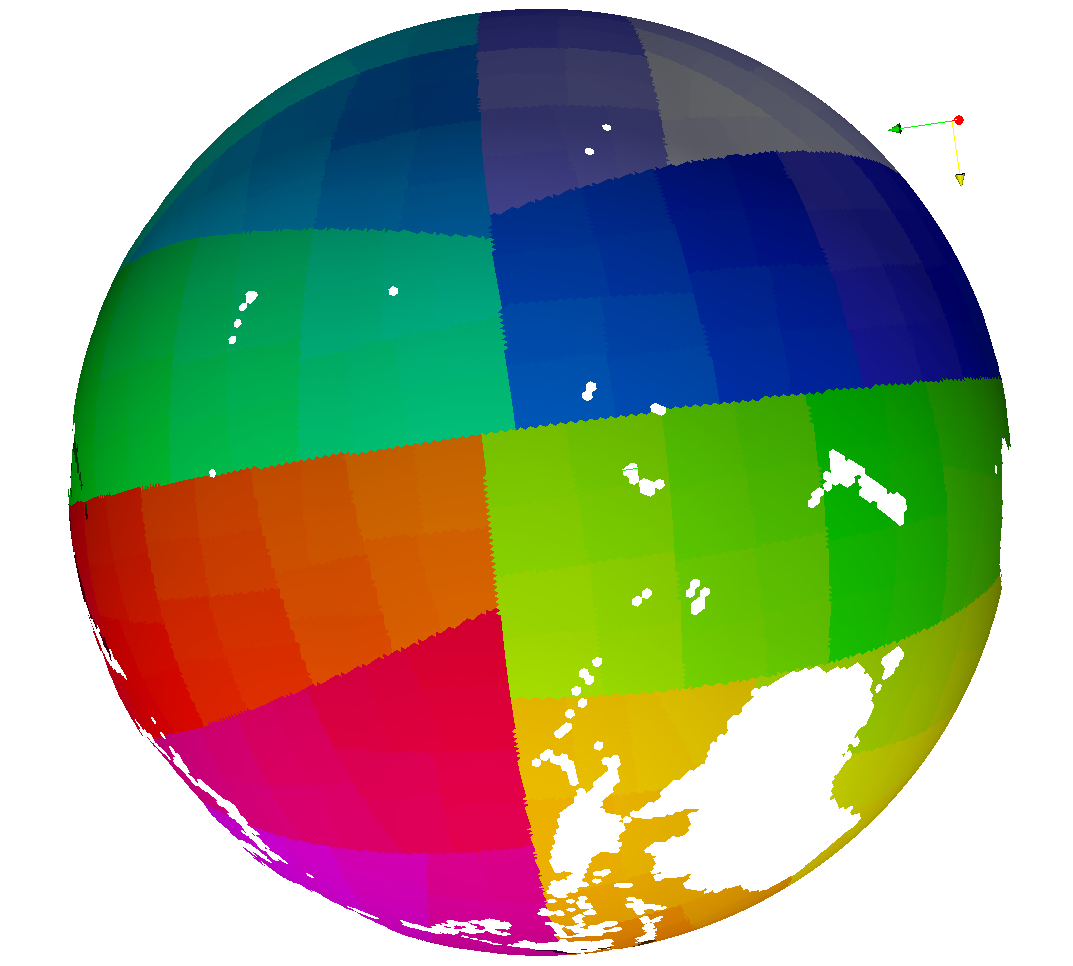
\includegraphics[width=0.45\textwidth]{60km/init/0_255.png}
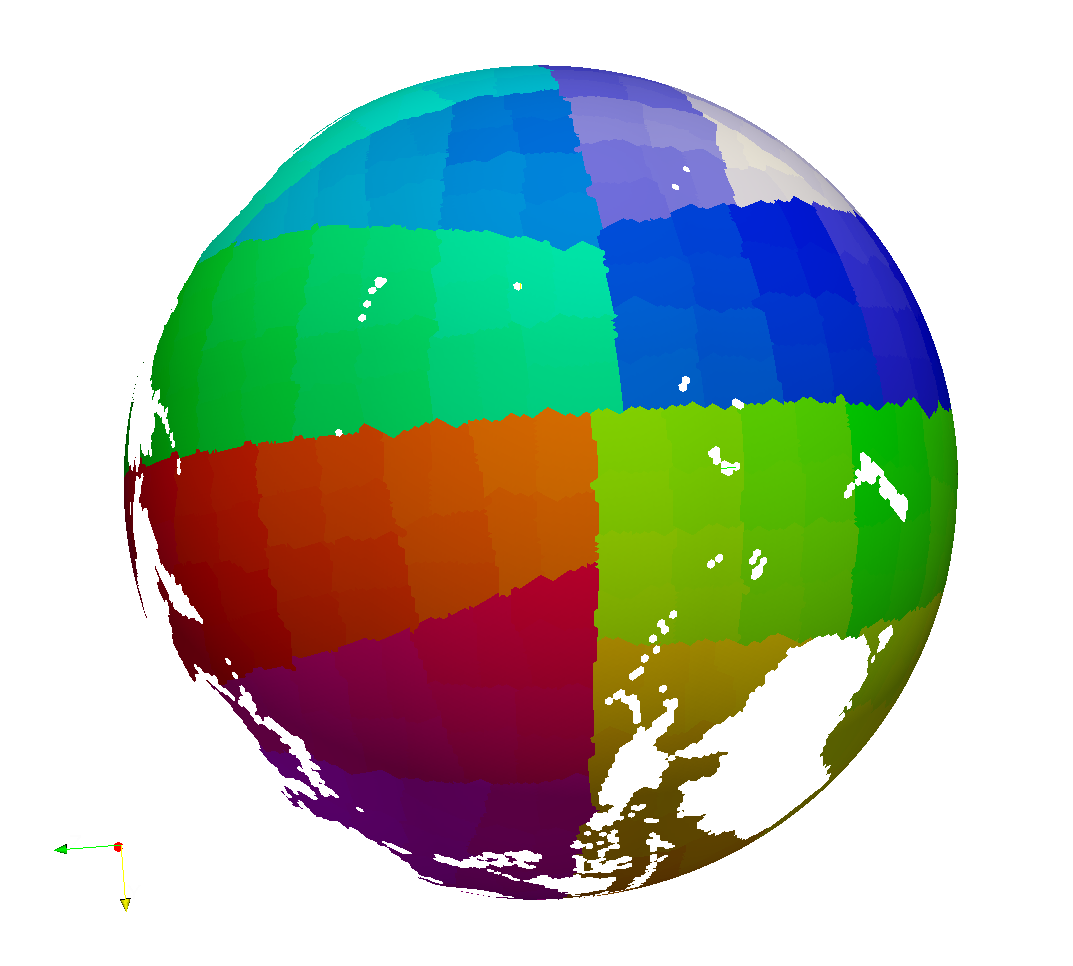
\includegraphics[width=0.5\textwidth]{60km/final/0_255.png}
\caption{\label{fig:60km0_255} RIB initial partition (left) and the ParMA ghost balanced partition (right).}
\end{figure}

\begin{figure} 
\centering
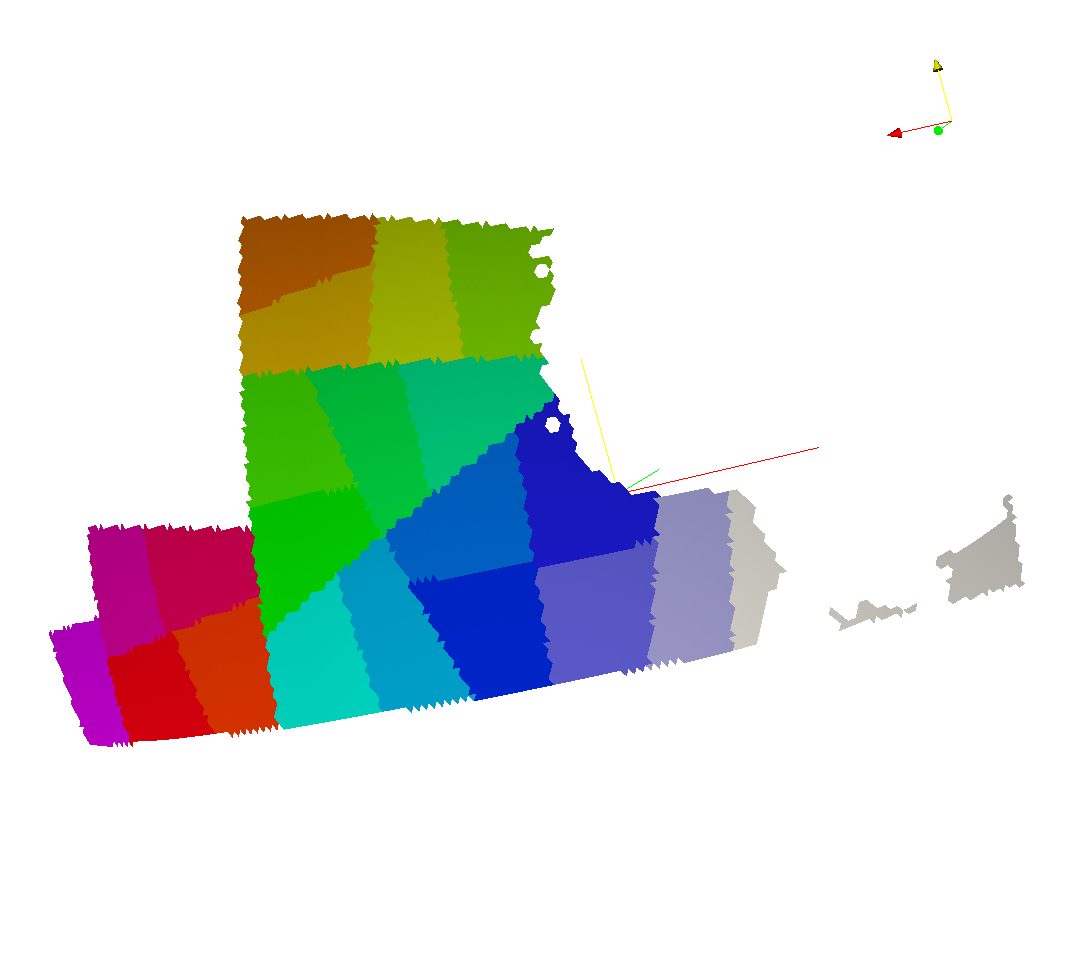
\includegraphics[width=0.8\textwidth]{60km/init/384_404.png}
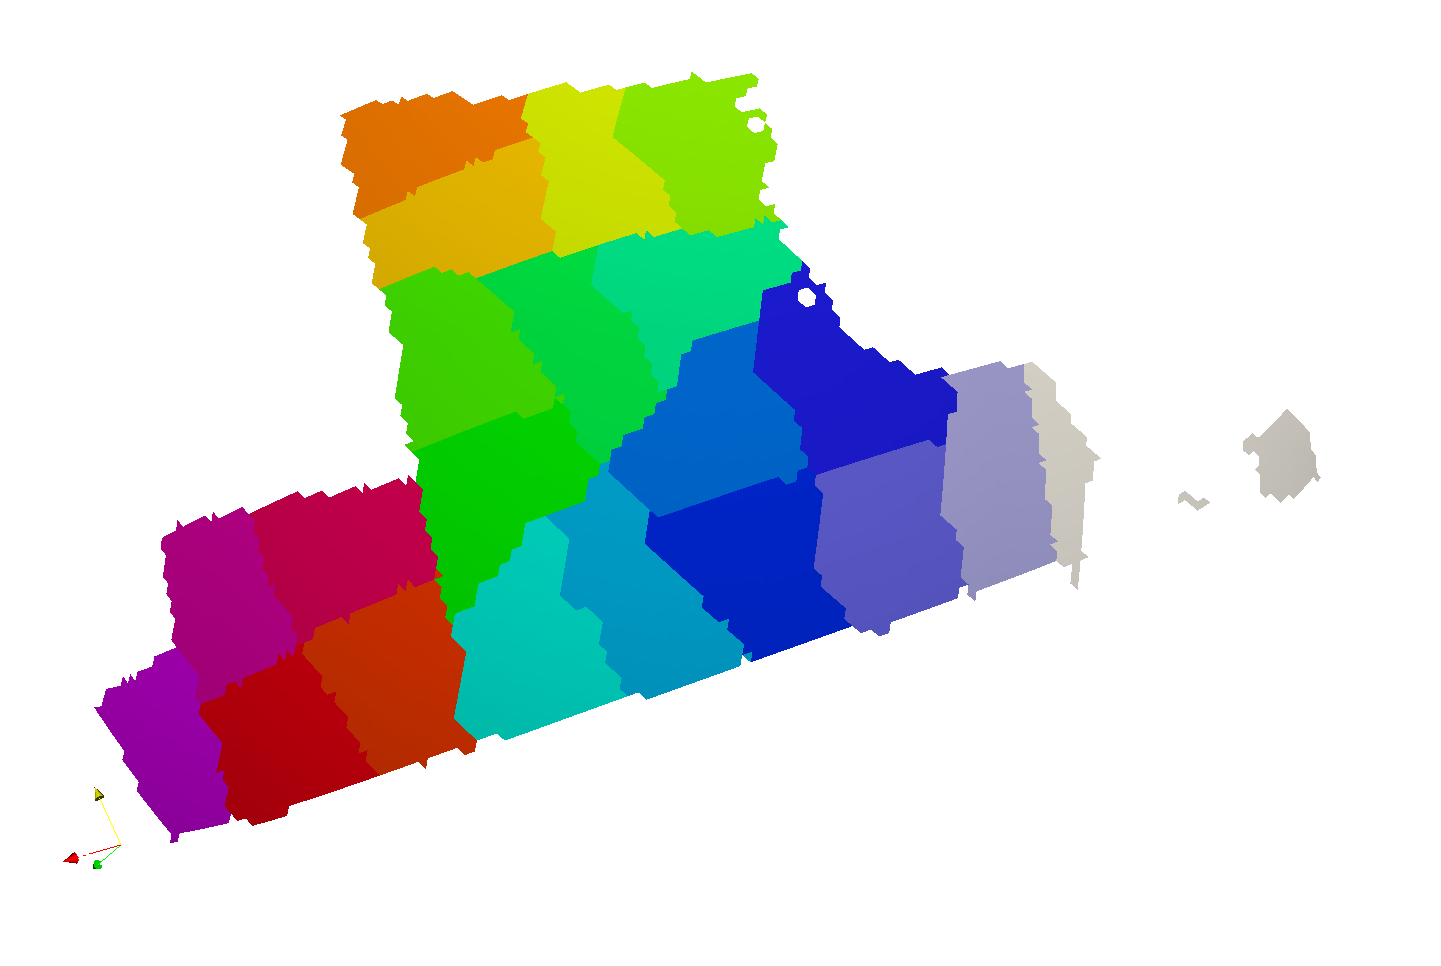
\includegraphics[width=0.8\textwidth]{60km/final/384_404.png}
\caption{\label{fig:60km384_404} RIB initial partition (top) and the ParMA ghost balanced partition (bottom).}
\end{figure}


\begin{algorithm}
\caption{ParMA Ghosting improvement}
\label{alg:parma}
\begin{algorithmic}[1]
\Require {mesh $M$ of dimension $d$, bridge ent dim $bDim$, num ghost layers $layers$}
\Procedure{parma}{$M$, $bDim$, $layers$}
  \While {$imbalance > tolerance$}
    \State $nbors \leftarrow findNeighbors()$
    \State //part weight only includes owned vertices
    \State $weight \leftarrow exchangeWeights(nbors)$
    \State //part weight only includes owned vertices
    \State $ghost \leftarrow exchangeGhostWeights(nbors)$
    \State $tgts \leftarrow computeTargets(weight, ghost)$
    \State $diffuse(tgts)$
  \EndWhile
\EndProcedure

\Procedure{diffuse(targets)}{}
  \State $plan \leftarrow \emptyset$
  \ForEach {$vtx \in boundaryVertices$}
    \State $neighbor \leftarrow getNeighbor(elm)$
    \If { $tgts.has(neighbor)$ AND $plan(neighbor) < tgts(neighbor)$}
      \If {meets selection criteria}
        \State $plan.add(elm)$
      \EndIf 
    \EndIf
  \EndFor
  \State $migrate(plan)$
\EndProcedure
\end{algorithmic}
\end{algorithm}

\section{Code}

The source can be downloaded from the following github repo \\
https://github.com/SCOREC/core

The code in parma/diffMC/src/parma\_ghost.cc implements the partitioning procedures and test/ghost.cc provides a test driver.  The test driver can be built with the command `make ghost'.  In the plate/2 directory of the test meshes SVN repo http://redmine.scorec.rpi.edu/svn/meshes is a two part 2D mesh for testing.  This mesh is classified on the plate/plate.dmg model.  Run the driver with the command `mpirun -np PROCS ./ghost MODEL MESH'.

\newpage
\bibliographystyle{plain}
\bibliography{references.bib}


\end{document}


